\documentclass{article}
\usepackage{amsmath}
\usepackage{xcolor}
\usepackage{gensymb}
\usepackage{ragged2e}
\usepackage{graphicx}
\usepackage{gensymb}
\usepackage{mathtools}
\newcommand{\mydet}[1]{\ensuremath{\begin{vmatrix}#1\end{vmatrix}}}
\providecommand{\brak}[1]{\ensuremath{\left(#1\right)}}
\providecommand{\norm}[1]{\left\lVert#1\right\rVert}
\newcommand{\solution}{\noindent \textbf{Solution: }}
\newcommand{\myvec}[1]{\ensuremath{\begin{pmatrix}#1\end{pmatrix}}}
\let\vec\mathbf
\begin{document}
\begin{center}
        \textbf\large{CHAPTER-9 \\ AREAS OF PARALLELOGRAMS AND TRIANGLES}
\end{center}
\section{Exercise 9.2}
Q1. In the figure given below, $ABCD$ is a parallelogram, $AE \perp DC$ and $CF \perp AD$.If $AB = 16cm$, $AE = 8cm$ and $CF = 10cm$, find $AD$.\\
\textbf{Construction}\\
\begin{figure}[h]
 \begin{center}
  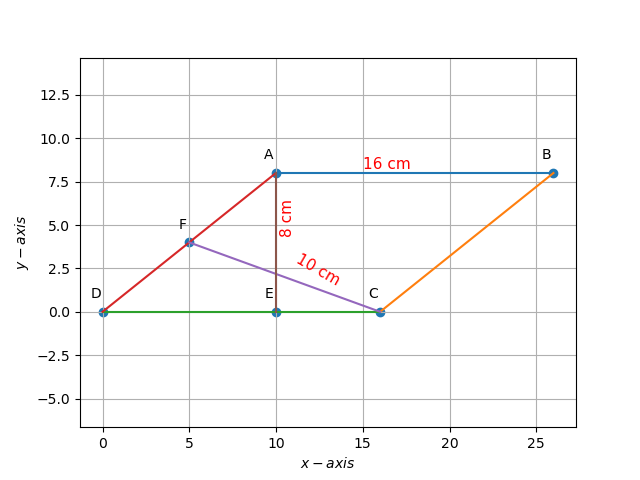
\includegraphics[width=\columnwidth]{fig1.png}
 \end{center}
 \caption{Parallelogram ABCD}
 \label{fig:Fig}
\end{figure}\\
\pagebreak
The input parameters for the above construction are shown in the table below : \\
\begin{table}[h]
	\centering
	\begin{tabular}{|c|c|c|}
\hline
Symbol & Value & Description\\
\hline
$x$ & 16cm & $\vec{AB}$ \\
\hline
$a$ & 10cm & $\vec{CF}$ \\
\hline
$b$ & 8cm & $\vec{AE}$ \\
\hline
$\angle{CFD}$ & $90\degree$ & $CF \perp AD$ \\
\hline
$\angle{AED}$ & $90\degree$ & $AE \perp CD$ \\
\hline
\end{tabular}

	\caption{Parameters}
	\label{tab:table1}
\end{table}\\
The input co-ordinates of the above parallelogram are given in this table : \\
\begin{table}[h]
	\centering
	\begin{tabular}{|p{2cm}|p{2cm}|p{2cm}|}
\hline
\multicolumn{3}{|c|}{Truth table}\\
\hline
R& S& A\\
\hline
0& 0& 0\\
\hline
0& 1& 1\\
\hline
1& 0& 1\\
\hline
1& 1& 0\\
\hline
\end{tabular}

	\caption{Co-ordinates}
	\label{tab:table2}
\end{table}\\
The rest of the co-ordinates were obtained in the following way : \\
\begin{enumerate}
\item Deriving the co-ordinates of A :\\
	A can be expressed in terms of (r$\cos{\theta}$,r$\sin{\theta}$).\\
To find out the value of r:\\
		From $\triangle{ADE}$, r is AD and $\theta$ is D.\\
		\begin{align}
		\sin{\theta} = \frac{AE}{AD}\\
		\implies \sin{\theta} = \frac{AE}{r}\\
			r = \frac{AE}{\sin{\theta}}\\
			r = \frac{8}{\sin{38.68}}\\
			r = 12.8cm\\
		\end{align}
The x co-ordinate is expressed as r$\cos{\theta}$.\\
		\begin{align}
			A_x = r * \cos{\theta}\\
			\implies (12.8) * (\cos{38.68}) = 10cm\\
		\end{align}
The y co-ordinate can be expressed as r$\sin{\theta}$.\\
		\begin{align}
			A_y = r * \sin{\theta}\\
			\implies (12.8) * (\sin{38.68}) = 8cm\\
		\end{align}
So, the co-ordinates of A are (10,8).
\item Deriving the co-ordinates for E :\\
The co-ordinates of E can be derived using a$e_1$, where a is the length of DE.To find out the length of DE we have to do the following steps : \\
		\begin{align}
			DE = \cos{D} * (AD) (from \triangle{ADE})\\
			DE = \cos{38.68} * (12.8) \\
			DE = 10cm = a\\
		\end{align}
Now E can be expresed as a*$e_1$ which is equal to
		\begin{center}
			10\myvec{1\\0}\\
			$\implies$\myvec{10\\0}\\
		\end{center}
So, the co-ordinates of E are (10,0).
\item Deriving the co-ordinates of B : \\
	The y co-ordinate of B is same as that of A because both the points are on the same horizontal line which is 8.\\
In order to obtain the x co-ordinate :
		\begin{align}
			B_x = A_x + 16(because \norm{\vec{AB}} = 16cm)\\
			B_x = 10 +16 = 26.\\
		\end{align}
The co-ordinates of B are (26,8).\\
\item Deriving the co-ordinates of F :\\
The co-ordinates of F can be derived by applying section formula : \\
The value of m = 12.48 and n = 0.32 and m : n = 39 : 1.\\
The co-ordinates of point D are cosidered to be ($x_1$,$y_1$) and co-ordinates of point A are considered to be ($x_2$,$y_2$).\\
The x co-ordinate is obtained using, \\
		\begin{align}
			F_x = \frac{m(x_2) + n(x_1)}{m + n}\\
			F_x = \frac{39(10) + 1(0)}{39 + 1}\\
			\implies \frac{390}{40} = 9.75\\
		\end{align}
The y co-ordinate can be found out using, \\
		\begin{align}
			F_y = \frac{m(y_2) + n(y_1)}{m + n}\\
			F_y = \frac{39(8) + 1(0)}{39 + 1}\\
			\implies \frac{312}{40} = 7.8 \\
		\end{align}
So, the co-ordinates of F are (9.75,7.8).
\end{enumerate}
\textbf{Solution}\\
It is given that the length of $AB = 16cm$.So,\\
\begin{align}
	\norm{\vec{B} - \vec{A}} = 16cm \\
\end{align}
As the figure above is a parallelogram,\\
\begin{align}
	\norm{\vec{B} - \vec{A}} = \norm{\vec{C} - \vec{D}} = 16cm
	\label{eq:3}\\
\end{align}
\vspace{5mm}
In order to find \angle{DCF},\\
\begin{align}
	\text{ Let }\theta_2 = \angle{FCD}\\
\vec{n_1} = &\vec{C} - \vec{F} = \myvec{6.25\\-7.806}, \vec{n_2} = \vec{C} - \vec{D} = \myvec{16\\0} \\
\theta_2 = &\cos^{-1}\frac{\vec{n_1}^\top\vec{n_2}}{\norm{\vec{n_1}}\norm{\vec{n_2}}} \\
	\implies\theta_2 = &\cos^{-1}\frac{\myvec{6.25&-7.806}\myvec{16\\0}}{(10)(16)} = 51.32\degree
\end{align}
As the sum of interal angles of a triangle are $180\degree$,from $\triangle{DFC}$\\
\begin{align}
	\angle{CFD} + \angle{FCD} + \angle{D} = 180\degree\\
	\angle{D} = 180\degree - (\angle{CFD} + \angle{FCD})\\
	\angle{D} = 180\degree - 141.32\degree \\
	\angle{D} = 38.68\degree
	\label{eq:4}\\
\end{align}
The area of parallelogram is calculated using the below formula\\
\begin{align}
	Area = (base)*(height)\\
\end{align}
For the above problem this can be written as,
\begin{align}
	Area = \norm{\vec{A} - \vec{E}} \norm{\vec{B} - \vec{A}}\\
	\implies (8) (16) = 128
	\label{eq:5}\\
\end{align}
The area of parallelogram can also be found out using cross product of two vectors,for the above problem it can be written as;
\begin{align}
	Area of parallelogram ABCD = \vec{DC} \times \vec{AD}\\
	\vec{DC} \times \vec{AD} = \norm{\vec{D} - \vec{C}} \norm{\vec{D} - \vec{A}} \sin{D}
	\label{eq:6}\\
\end{align}
From \ref{eq:3} and \ref{eq:6}\\
\begin{align}
	\norm{\vec{D} - \vec{A}} (16) \sin{38.68} = 128\\
	\norm{\vec{D} - \vec{A}} (16) (\frac{5}{8}) = 128\\
	\norm{\vec{D} - \vec{A}} = \frac{64}{5}\\
	\norm{\vec{D} - \vec{A}} = 12.8cm\\
\end{align}
Therefore,$|\hspace{0.1cm}$\textbf{$\overrightarrow{\vec{AD}}\hspace{0.1cm} |$ = 12.8 cm}\\
\end{document}




